\documentclass[tikz,border=5mm]{standalone}
\usepackage{pgfplots}
\pgfplotsset{compat=1.17}

\begin{document}
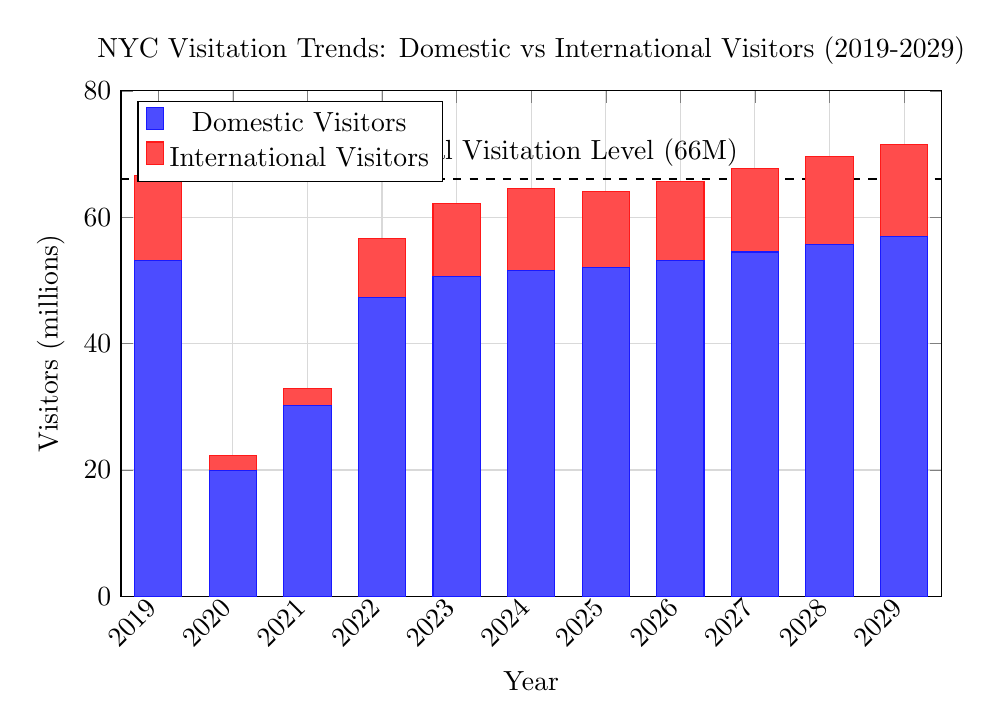
\begin{tikzpicture}
\begin{axis}[
    width=12cm,
    height=8cm,
    ybar stacked,
    bar width=0.6cm,
    xlabel={Year},
    ylabel={Visitors (millions)},
    title={NYC Visitation Trends: Domestic vs International Visitors (2019-2029)},
    xmin=2018.5,
    xmax=2029.5,
    ymin=0,
    ymax=80,
    xtick={2019,2020,2021,2022,2023,2024,2025,2026,2027,2028,2029},
    xticklabels={2019,2020,2021,2022,2023,2024,2025,2026,2027,2028,2029},
    legend style={at={(0.02,0.98)}, anchor=north west},
    grid=major,
    grid style={gray!30},
    x tick label style={rotate=45, anchor=east},
]

% Domestic visitors data
\addplot[fill=blue!70, draw=blue!90] coordinates {
    (2019,53.1) (2020,19.9) (2021,30.2) (2022,47.3) (2023,50.6) 
    (2024,51.6) (2025,52.0) (2026, 53.1) (2027,54.5) (2028,55.7) (2029,56.9)
};

% International visitors data
\addplot[fill=red!70, draw=red!90] coordinates {
    (2019,13.5) (2020,2.4) (2021,2.7) (2022,9.4) (2023,11.6) 
    (2024,12.9) (2025,12.1) (2026,12.5) (2027,13.2) (2028,13.9) (2029,14.6)
};

% Horizontal dashed line for 2019 total visitation level
\draw[dashed, thick, color=black] (axis cs:2018.5,66) -- (axis cs:2029.5,66);
\node[anchor=south] at (axis cs:2024,66.5) {2019 Total Visitation Level (66M)};

\legend{Domestic Visitors, International Visitors}

\end{axis}
\end{tikzpicture}
\end{document}